% ============================================================
%  Lecture 2 — Expanding Universe and Background Dynamics
%  Beamer slide deck
% ============================================================
\documentclass[aspectratio=169,11pt]{beamer}

% --- Theme --------------------------------------------------
\usetheme{Madrid}
\usecolortheme{default}
\setbeamertemplate{navigation symbols}{}
\setbeamertemplate{footline}[frame number]

% --- Packages -----------------------------------------------
\usepackage{amsmath,amssymb,mathtools}
\usepackage{bm}
\usepackage{graphicx}
\graphicspath{{../notes/figures/}}
\usepackage{booktabs}
\usepackage{tikz}
\usepackage[export]{adjustbox}

% --- Macros (from notes/preamble.tex) -----------------------
\newcommand{\dd}{\mathrm{d}}
\newcommand{\ee}{\mathrm{e}}
\newcommand{\Omm}{\Omega_{\mathrm{m}}}
\newcommand{\Omr}{\Omega_{\mathrm{r}}}
\newcommand{\Omk}{\Omega_{k}}
\newcommand{\Omtot}{\Omega_{\mathrm{tot}}}
\newcommand{\OmDE}{\Omega_{\mathrm{DE}}}
\newcommand{\Lcdm}{\Lambda\mathrm{CDM}}
\newcommand{\Hnot}{H_0}
\newcommand{\kmsMpc}{\,\mathrm{km\,s^{-1}\,Mpc^{-1}}}

% --- Title --------------------------------------------------
\title{Expanding Universe and Background Dynamics}
\subtitle{Lecture 2}
\author{Dr.\ Cristiano Sabiu}
\institute{Natural Science Research Institute\\University of Seoul}
\date{\today}


% ============================================================
\begin{document}

% ---- Slide 1: Title ----------------------------------------
\begin{frame}[plain]
\titlepage
\end{frame}

% ---- Slide 2: Outline --------------------------------------
\begin{frame}{Outline}
\tableofcontents
\end{frame}


% ============================================================
\section{Tensor Algebra Interlude}
% ============================================================

% ---- Slide 3 -----------------------------------------------
\begin{frame}{Index Notation and Einstein Summation}
\begin{itemize}
    \item Greek indices $\mu,\nu,\ldots = 0,1,2,3$ (spacetime)
    \item Latin indices $i,j,\ldots = 1,2,3$ (spatial only)
    \item \textbf{Einstein summation convention:} repeated upper+lower index $\Rightarrow$ sum
\end{itemize}
\begin{equation*}
    A^\mu B_\mu \equiv \sum_{\mu=0}^{3} A^\mu B_\mu
    = A^0 B_0 + A^1 B_1 + A^2 B_2 + A^3 B_3
\end{equation*}
\begin{itemize}
    \item Repeated index = \emph{dummy} (summed); single index = \emph{free}
\end{itemize}
\end{frame}

% ---- Slide 4 -----------------------------------------------
\begin{frame}{The Metric Tensor $g_{\mu\nu}$}
\begin{itemize}
    \item Defines the invariant interval between neighbouring events:
\end{itemize}
\begin{equation*}
    ds^2 = g_{\mu\nu}\,dx^\mu\,dx^\nu
\end{equation*}
\begin{itemize}
    \item Symmetric: $g_{\mu\nu}=g_{\nu\mu}$
    \item Inverse: $g^{\mu\alpha}g_{\alpha\nu}=\delta^\mu_{\ \nu}$
    \item \textbf{Raises indices:} $V^\mu = g^{\mu\nu}V_\nu$
    \item \textbf{Lowers indices:} $V_\mu = g_{\mu\nu}V^\nu$
    \item $V^\mu$ and $V_\mu$ are the same geometric object in two representations
\end{itemize}
\end{frame}

% ---- Slide 5 -----------------------------------------------
\begin{frame}{Contraction}
\begin{itemize}
    \item \textbf{Contraction:} set an upper and lower index equal and sum (take a trace)
    \item From a rank-2 tensor $T^\mu_{\ \nu}$, the contraction $T^\mu_{\ \mu}$ is a scalar
    \item Example --- the Ricci scalar:
\end{itemize}
\begin{equation*}
    R = g^{\mu\nu}R_{\mu\nu}
\end{equation*}
\vfill
\begin{center}
\structure{These conventions are all we need for the GR derivation that follows.}
\end{center}
\end{frame}


% ============================================================
\section{Friedmann via General Relativity}
% ============================================================

% ---- Slide 6 -----------------------------------------------
\begin{frame}{The Role of the Metric}
\begin{itemize}
    \item The metric tells you how to compute distances and time intervals
    \item Familiar example --- Minkowski metric (flat, static):
\end{itemize}
\begin{equation*}
    ds^2 = -c^2\,dt^2 + dx^2 + dy^2 + dz^2
\end{equation*}
\begin{itemize}
    \item Constant coefficients $\Rightarrow$ no gravity, no expansion
    \item GR generalises: coefficients become functions of coordinates
\begin{equation*}
    ds^2 = g_{\mu\nu}\,dx^\mu\,dx^\nu
\end{equation*}
    \item For cosmology: coefficients depend on time through $a(t)$
\end{itemize}
\end{frame}

% ---- Slide 7 -----------------------------------------------
\begin{frame}{The Cosmological Principle}
\begin{block}{Cosmological Principle}
The universe is \textbf{spatially homogeneous} (no preferred location) and \textbf{isotropic} (no preferred direction) on sufficiently large scales.
\end{block}
\vspace{0.3cm}
\textbf{Observational support:}
\begin{itemize}
    \item Large-scale galaxy distribution
    \item CMB isotropy: $\delta T/T \sim 10^{-5}$
    \item Isotropic Hubble flow
\end{itemize}
\vspace{0.3cm}
\begin{equation*}
    \text{Einstein's Field Equations} + \text{Cosmological Principle}
    \;\Longrightarrow\; \text{FLRW Metric}
\end{equation*}
\end{frame}

% ---- Slide 8 -----------------------------------------------
\begin{frame}{Historical Development}
\begin{description}
    \item[Friedmann (1922, 1924)] First dynamical solutions --- universe need not be static
    \item[Lema\^{i}tre (1927)] Independently derived expanding solution; proposed linear $v$--$d$ relation \emph{before} Hubble (1929)
    \item[Robertson (1935--36) \& Walker (1937)] Rigorous proof: homogeneity + isotropy \emph{uniquely} determine the metric form
\end{description}
\vfill
\small The metric carries four names because it was assembled in stages over two decades.
\end{frame}

% ---- Slide 9 -----------------------------------------------
\begin{frame}{The FLRW Metric}
\begin{alertblock}{FLRW Line Element}
\begin{equation*}
    ds^{2} = -c^{2}\,dt^{2}
    + a^{2}(t)\!\left[\frac{dr^{2}}{1-kr^{2}}
    + r^{2}\!\left(d\theta^{2} + \sin^{2}\!\theta\;d\phi^{2}\right)\right]
\end{equation*}
\end{alertblock}
\begin{itemize}
    \item $t$ = cosmic time (proper time of comoving observers)
    \item $a(t)$ = scale factor; $a(t_0)=1$ today
    \item $k=+1$ (closed), $0$ (flat), $-1$ (open)
    \item $r$ = comoving radial coordinate; physical distance $= a(t)\cdot r$
\end{itemize}
\end{frame}

% ---- Slide 10 ----------------------------------------------
\begin{frame}{FLRW Metric Components}
Non-zero components:
\begin{equation*}
    g_{00}=-c^2,\quad g_{rr}=\frac{a^2}{1-kr^2},\quad
    g_{\theta\theta}=a^2r^2,\quad g_{\phi\phi}=a^2r^2\sin^2\!\theta
\end{equation*}
Inverses:
\begin{equation*}
    g^{00}=-\frac{1}{c^2},\quad g^{rr}=\frac{1-kr^2}{a^2},\quad
    g^{\theta\theta}=\frac{1}{a^2r^2},\quad g^{\phi\phi}=\frac{1}{a^2r^2\sin^2\!\theta}
\end{equation*}
\vfill
\footnotesize\textbf{Convention:} From here on we adopt \textbf{natural units} $c=1$ for the GR derivation. This keeps the algebra clean; we restore $c$ where needed later.
\end{frame}

% ---- Slide 11 ----------------------------------------------
\begin{frame}{Christoffel Symbols: Definition}
\begin{itemize}
    \item Encode how coordinate basis vectors change in curved spacetime
    \item Defined entirely from the metric and its first derivatives:
\end{itemize}
\begin{equation*}
    \Gamma^\mu_{\alpha\beta}
    = \frac{1}{2}\,g^{\mu\nu}\bigl(
    \partial_\alpha g_{\nu\beta}
    + \partial_\beta g_{\nu\alpha}
    - \partial_\nu g_{\alpha\beta}\bigr)
\end{equation*}
\begin{itemize}
    \item Diagonal FLRW metric simplifies the computation considerably
    \item \structure{Full calculation: see lecture notes --- here we state the key results}
\end{itemize}
\end{frame}

% ---- Slide 12 ----------------------------------------------
\begin{frame}{Christoffel Symbols: Key Results}
\begin{block}{Non-vanishing FLRW Christoffel symbols}
\begin{align*}
    \Gamma^0_{ij} &= H\,g_{ij}
        &&\text{(spatial metric changes with time)}\\[6pt]
    \Gamma^i_{0j} &= H\,\delta^i_{\ j}
        &&\text{(basis vectors stretched by expansion)}\\[6pt]
    \Gamma^i_{jk} &: \text{standard spherical + curvature terms}
\end{align*}
\end{block}
\begin{itemize}
    \item $H\equiv\dot{a}/a$ is the \textbf{Hubble parameter}
    \item All other Christoffel symbols vanish: $\Gamma^0_{00}=\Gamma^0_{0i}=\Gamma^i_{00}=0$
\end{itemize}
\end{frame}

% ---- Slide 13 ----------------------------------------------
\begin{frame}{The Ricci Tensor}
\begin{equation*}
    R_{\mu\nu}
    = \partial_\lambda\Gamma^\lambda_{\mu\nu}
    - \partial_\nu\Gamma^\lambda_{\mu\lambda}
    + \Gamma^\lambda_{\lambda\sigma}\Gamma^\sigma_{\mu\nu}
    - \Gamma^\lambda_{\nu\sigma}\Gamma^\sigma_{\mu\lambda}
\end{equation*}
\vspace{0.3cm}
\textbf{Strategy --- exploit FLRW symmetry:}
\begin{itemize}
    \item Isotropy $\Rightarrow$ $R_{0i}=0$
    \item Homogeneity + isotropy $\Rightarrow$ $R_{ij}=f(t)\,g_{ij}$
    \item We only need to compute $R_{00}$ and one function $f(t)$
\end{itemize}
\end{frame}

% ---- Slide 14 ----------------------------------------------
\begin{frame}{Ricci Tensor: Results}
Evaluating the four terms for $R_{00}$ and $R_{ij}$:

\begin{alertblock}{$R_{00}$}
\vspace{-0.1cm}
\begin{equation*}
    R_{00} = -3\,\frac{\ddot{a}}{a}
\end{equation*}
\vspace{-0.3cm}
\end{alertblock}
\begin{itemize}
    \item Independent of spatial curvature $k$
\end{itemize}

\begin{alertblock}{$R_{ij}$}
\vspace{-0.1cm}
\begin{equation*}
    R_{ij} = \left(\frac{\ddot{a}}{a} + 2H^2 + \frac{2k}{a^2}\right)g_{ij}
\end{equation*}
\vspace{-0.3cm}
\end{alertblock}
\begin{itemize}
    \item \structure{Full four-term evaluation for each: see lecture notes}
\end{itemize}
\end{frame}

% ---- Slide 15 ----------------------------------------------
\begin{frame}{Ricci Scalar and Einstein Tensor}
\begin{columns}[T]
\column{0.48\textwidth}
\begin{block}{Ricci Scalar}
\begin{equation*}
    R = 6\!\left(\frac{\ddot{a}}{a} + H^2 + \frac{k}{a^2}\right)
\end{equation*}
\end{block}

\column{0.48\textwidth}
\begin{block}{Einstein Tensor $G_{00}$}
\begin{equation*}
    G_{00} = 3\!\left(H^2+\frac{k}{a^2}\right)
\end{equation*}
\end{block}
\end{columns}

\vspace{0.5cm}
\begin{itemize}
    \item $G_{\mu\nu}=R_{\mu\nu}-\frac{1}{2}g_{\mu\nu}R$
    \item The $\ddot{a}$ terms \textbf{cancel} in $G_{00}$ --- this is a \emph{constraint equation}
    \item $\nabla^\mu G_{\mu\nu}=0$ (Bianchi identity) ensures energy--momentum conservation
\end{itemize}
\end{frame}

% ---- Slide 16 ----------------------------------------------
\begin{frame}{Energy--Momentum Tensor: Perfect Fluid}
\begin{itemize}
    \item Homogeneity + isotropy require a \textbf{perfect fluid}
    \item Characterised by energy density $\rho$ and pressure $p$
\end{itemize}
\begin{equation*}
    T^\mu_{\ \nu}
    = \mathrm{diag}(-\rho c^2,\; p,\; p,\; p)
\end{equation*}
Lowering an index with $g_{\mu\lambda}$:
\begin{equation*}
    T_{00} = \rho c^2, \qquad T_{ij} = p\,g_{ij}
\end{equation*}
\end{frame}

% ---- Slide 17 ----------------------------------------------
\begin{frame}{Einstein Field Equations}
\begin{alertblock}{Einstein Field Equations}
\begin{equation*}
    G_{\mu\nu} = 8\pi G\,T_{\mu\nu}
\end{equation*}
\end{alertblock}
\vspace{0.3cm}
\begin{center}
\large\textbf{Geometry = Matter content}
\end{center}
\vspace{0.3cm}
\begin{itemize}
    \item Left side: curvature of spacetime ($G_{\mu\nu}$)
    \item Right side: energy and momentum of matter ($T_{\mu\nu}$)
    \item Now we plug in our FLRW results\ldots
\end{itemize}
\end{frame}

% ---- Slide 18 ----------------------------------------------
\begin{frame}{The First Friedmann Equation}
From $G_{00}=8\pi G\,T_{00}$:
\begin{equation*}
    3H^2 + \frac{3k}{a^2} = 8\pi G\,\rho
\end{equation*}

\begin{alertblock}{First Friedmann Equation}
\begin{equation*}
    H^2 = \left(\frac{\dot{a}}{a}\right)^{\!2}
    = \frac{8\pi G}{3}\,\rho - \frac{k}{a^2}
\end{equation*}
\end{alertblock}

\begin{itemize}
    \item Governs the \textbf{expansion rate} of the Universe
    \item A \emph{constraint} equation (no $\ddot{a}$)
\end{itemize}
\end{frame}

% ---- Slide 19 ----------------------------------------------
\begin{frame}{Critical Density and $\Omega$}
For $k=0$, the expansion rate is set solely by the energy density. Define the \textbf{critical density}:
\begin{equation*}
    \rho_{\rm crit} \equiv \frac{3H^2}{8\pi G}
\end{equation*}
\textbf{Density parameter} for component $i$:
\begin{equation*}
    \Omega_i \equiv \frac{\rho_i}{\rho_{\rm crit}}
\end{equation*}
Curvature parameter: $\Omk\equiv -k/(aH)^2$

\vspace{0.3cm}
\begin{block}{Friedmann equation in $\Omega$ language}
\begin{equation*}
    \Omtot + \Omk = 1
\end{equation*}
\end{block}
Observations: $|\Omk|\lesssim 10^{-3}$ --- the Universe is very close to flat.
\end{frame}

% ---- Slide 20 ----------------------------------------------
\begin{frame}{The Second Friedmann Equation}
From the spatial components of $G_{\mu\nu}=8\pi G\,T_{\mu\nu}$:

\begin{alertblock}{Second Friedmann Equation (Acceleration / Raychaudhuri)}
\begin{equation*}
    \frac{\ddot{a}}{a} = -\frac{4\pi G}{3}\,(\rho+3p)
\end{equation*}
\end{alertblock}

\begin{itemize}
    \item Independent of $k$
    \item $\rho+3p>0$ (matter, radiation) $\Rightarrow$ $\ddot{a}<0$: \textbf{deceleration}
    \item Accelerating expansion requires $p<-\rho/3$ --- \textbf{dark energy!}
\end{itemize}
\end{frame}

% ---- Slide 21 ----------------------------------------------
\begin{frame}{Conformal Time}
Define \textbf{conformal time} $\eta$ by $\dd\eta = \dd t/a(t)$. The FLRW metric becomes ($k=0$):
\begin{equation*}
    ds^2 = a^2(\eta)\!\left[-c^2\,d\eta^2 + d\chi^2 + \chi^2\,d\Omega^2\right]
\end{equation*}

\begin{columns}[T]
\column{0.55\textwidth}
\begin{itemize}
    \item Light cones are $45^\circ$ lines on a $\chi$--$\eta$ diagram
    \item Essential for causal structure, CMB physics, and perturbation theory
\end{itemize}

\column{0.4\textwidth}
% TODO: Add figure --- conformal spacetime diagram showing
% light cones as 45-degree lines on a chi-eta diagram
\begin{center}
\textit{[Figure: conformal diagram]}
\end{center}
\end{columns}
\end{frame}


% ============================================================
\section{Newtonian Derivation}
% ============================================================

% ---- Slide 22 ----------------------------------------------
\begin{frame}{Newtonian Derivation: Setup}
\begin{columns}[T]
\column{0.55\textwidth}
\begin{itemize}
    \item Homogeneous, isotropic universe of uniform density $\rho(t)$
    \item Consider a thin shell of mass $m$ at radius
\begin{equation*}
    r(t) = a(t)\,r_0
\end{equation*}
    \item Shell theorem: only interior mass contributes
\begin{equation*}
    M = \tfrac{4}{3}\pi r^3\rho
\end{equation*}
\end{itemize}

\column{0.4\textwidth}
\centering
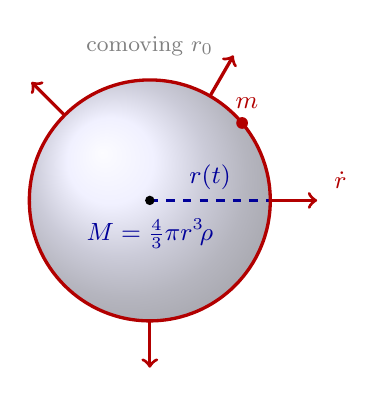
\begin{tikzpicture}[scale=0.85]
  % Filled interior (shaded sphere)
  \shade[ball color=blue!15, opacity=0.5] (0,0) circle (1.8);
  % Dashed interior radius
  \draw[dashed, thick, blue!60!black] (0,0) -- node[above,font=\small]{$r(t)$} (1.8,0);
  % Shell (thick circle)
  \draw[very thick, red!70!black] (0,0) circle (1.8);
  % Centre dot
  \fill (0,0) circle (2pt);
  % Mass label on shell
  \node[red!70!black, font=\small\bfseries] at (1.45,1.45) {$m$};
  % Small dot on shell
  \fill[red!70!black] ({1.8*cos(40)},{1.8*sin(40)}) circle (2.5pt);
  % Enclosed mass label
  \node[blue!60!black, font=\small] at (0,-0.5) {$M=\tfrac{4}{3}\pi r^3\!\rho$};
  % Outward arrow (expansion)
  \draw[->, very thick, red!70!black] (1.8,0) -- (2.5,0);
  \draw[->, very thick, red!70!black] ({1.8*cos(60)},{1.8*sin(60)})
    -- ({2.5*cos(60)},{2.5*sin(60)});
  \draw[->, very thick, red!70!black] ({1.8*cos(135)},{1.8*sin(135)})
    -- ({2.5*cos(135)},{2.5*sin(135)});
  \draw[->, very thick, red!70!black] (0,-1.8) -- (0,-2.5);
  % Velocity label
  \node[red!70!black, font=\small] at (2.85,0.3) {$\dot{r}$};
  % Comoving label
  \node[font=\footnotesize, gray] at (0,2.3) {comoving $r_0$};
\end{tikzpicture}
\end{columns}
\end{frame}

% ---- Slide 23 ----------------------------------------------
\begin{frame}{First Friedmann from Energy Conservation}
Kinetic energy: $T = \frac{1}{2}m\dot{a}^2r_0^2$

Potential energy: $U = -\frac{4\pi G}{3}\,m\,a^2r_0^2\,\rho$

\vspace{0.2cm}
Energy conservation: $T+U=E=\text{const}$

\vspace{0.2cm}
Divide by $\frac{1}{2}ma^2r_0^2$ and define $k\equiv-2E/(mr_0^2)$:

\begin{alertblock}{First Friedmann Equation (Newtonian)}
\begin{equation*}
    H^2 = \frac{8\pi G}{3}\,\rho - \frac{k}{a^2}
\end{equation*}
\end{alertblock}
\alert{Same as the GR result!}
\end{frame}

% ---- Slide 24 ----------------------------------------------
\begin{frame}{Interpretation of $k$}
The constant $k$ is related to the total energy of the shell:
\vspace{0.3cm}
\begin{itemize}
    \item<1-> $E<0\;\Rightarrow\;k>0$: gravitationally bound $\longrightarrow$ \textbf{closed} universe
    \item<2-> $E=0\;\Rightarrow\;k=0$: exact escape energy $\longrightarrow$ \textbf{flat} universe
    \item<3-> $E>0\;\Rightarrow\;k<0$: unbound $\longrightarrow$ \textbf{open} universe
\end{itemize}
\vspace{0.5cm}
\uncover<4->{%
\structure{The Newtonian energy constant maps directly onto the GR curvature parameter.}}
\end{frame}

% ---- Slide 25 ----------------------------------------------
\begin{frame}{Second Friedmann from Newton's Second Law}
Gravitational acceleration of the shell:
\begin{equation*}
    \ddot{r} = -\frac{GM}{r^2}
\end{equation*}
Substitute $r=ar_0$, $M=\tfrac{4}{3}\pi a^3 r_0^3\rho$:
\begin{equation*}
    \frac{\ddot{a}}{a} = -\frac{4\pi G}{3}\,\rho
    \qquad\text{(Newtonian)}
\end{equation*}
\vspace{0.3cm}
\structure{GR correction:} pressure also gravitates ---
\begin{equation*}
    \frac{\ddot{a}}{a} = -\frac{4\pi G}{3}\,(\rho+3p)
    \qquad\text{(General Relativity)}
\end{equation*}
\end{frame}

% ---- Slide 26 ----------------------------------------------
\begin{frame}{GR vs.\ Newtonian: Summary}
\begin{columns}[T]
\column{0.46\textwidth}
\begin{block}{Newtonian}
\begin{align*}
    H^2 &= \frac{8\pi G}{3}\rho - \frac{k}{a^2}\\[8pt]
    \frac{\ddot{a}}{a} &= -\frac{4\pi G}{3}\,\rho
\end{align*}
\end{block}

\column{0.46\textwidth}
\begin{block}{General Relativity}
\begin{align*}
    H^2 &= \frac{8\pi G}{3}\rho - \frac{k}{a^2}\\[8pt]
    \frac{\ddot{a}}{a} &= -\frac{4\pi G}{3}(\rho+3p)
\end{align*}
\end{block}
\end{columns}

\vspace{0.4cm}
\begin{itemize}
    \item First Friedmann: \textbf{identical} in both
    \item Second Friedmann: GR adds the $3p$ pressure term
    \item GR is needed for: pressure contribution, $\Lambda$, radiation era, causal structure
\end{itemize}
\end{frame}


% ============================================================
\section{The Continuity Equation}
% ============================================================

% ---- Slide 27 ----------------------------------------------
\begin{frame}{The Fluid (Continuity) Equation}
Combine the two Friedmann equations: multiply 1st by $a^2$, differentiate, substitute 2nd.
\begin{alertblock}{Continuity Equation}
\begin{equation*}
    \dot{\rho} + 3H\!\left(\rho + \frac{p}{c^2}\right) = 0
\end{equation*}
\end{alertblock}
\begin{itemize}
    \item The curvature $k$ drops out (useful consistency check)
    \item Physical meaning: energy density changes because expansion does $p\,dV$ work
\end{itemize}
\end{frame}

% ---- Slide 28 ----------------------------------------------
\begin{frame}{Equation of State and Scaling}
Parametrise pressure: $p = w\rho c^2$ with constant $w$.

\vspace{0.2cm}
Continuity equation becomes: $\dot{\rho}+3(1+w)H\rho=0$

\vspace{0.3cm}
Integrates to:
\begin{alertblock}{General scaling relation}
\begin{equation*}
    \rho \propto a^{-3(1+w)}
\end{equation*}
\end{alertblock}
The value of $w$ determines how quickly the density dilutes with expansion.
\end{frame}

% ---- Slide 29 ----------------------------------------------
\begin{frame}{Matter (Dust): $w=0$}
\begin{columns}[T]
\column{0.55\textwidth}
\begin{equation*}
    \rho_m \propto a^{-3}
\end{equation*}
\begin{itemize}
    \item Fixed number of particles, diluted by growing volume $V\propto a^3$
    \item Mass of individual particles unchanged
    \item Simple volume dilution
\end{itemize}

\column{0.4\textwidth}
\centering
\vspace{0.3cm}
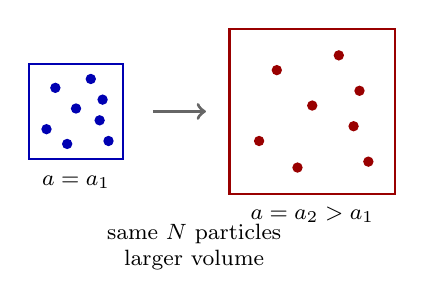
\begin{tikzpicture}[scale=0.75]
  % --- Small box (early time) ---
  \draw[thick, blue!70!black] (-0.8,-0.8) rectangle (0.8,0.8);
  % particles (dots)
  \fill[blue!70!black] (-0.35, 0.4) circle (2.5pt);
  \fill[blue!70!black] ( 0.25, 0.55) circle (2.5pt);
  \fill[blue!70!black] (-0.5,-0.3) circle (2.5pt);
  \fill[blue!70!black] ( 0.4,-0.15) circle (2.5pt);
  \fill[blue!70!black] ( 0.0, 0.05) circle (2.5pt);
  \fill[blue!70!black] (-0.15,-0.55) circle (2.5pt);
  \fill[blue!70!black] ( 0.45, 0.2) circle (2.5pt);
  \fill[blue!70!black] ( 0.55,-0.5) circle (2.5pt);
  % label
  \node[font=\footnotesize] at (0,-1.2) {$a=a_1$};

  % --- Arrow ---
  \draw[->, very thick, black!60] (1.3,0) -- (2.2,0);

  % --- Large box (later time) ---
  \begin{scope}[xshift=4cm]
  \draw[thick, red!60!black] (-1.4,-1.4) rectangle (1.4,1.4);
  % same particles, spread out
  \fill[red!60!black] (-0.6, 0.7) circle (2.5pt);
  \fill[red!60!black] ( 0.45, 0.95) circle (2.5pt);
  \fill[red!60!black] (-0.9,-0.5) circle (2.5pt);
  \fill[red!60!black] ( 0.7,-0.25) circle (2.5pt);
  \fill[red!60!black] ( 0.0, 0.1) circle (2.5pt);
  \fill[red!60!black] (-0.25,-0.95) circle (2.5pt);
  \fill[red!60!black] ( 0.8, 0.35) circle (2.5pt);
  \fill[red!60!black] ( 0.95,-0.85) circle (2.5pt);
  % label
  \node[font=\footnotesize] at (0,-1.75) {$a=a_2>a_1$};
  \end{scope}

  % Annotation
  \node[font=\footnotesize, text width=3cm, align=center]
    at (2.0, -2.3) {same $N$ particles\\larger volume};
\end{tikzpicture}
\end{columns}
\end{frame}

% ---- Slide 30 ----------------------------------------------
\begin{frame}{Radiation: $w=1/3$}
\begin{equation*}
    \rho_r \propto a^{-4}
\end{equation*}

\textbf{Two effects:}
\begin{enumerate}
    \item<1-> \textbf{Dilution:} number density $n\propto a^{-3}$ (same as matter)
    \item<2-> \textbf{Redshift:} wavelength stretches $\lambda\propto a$, so $E=hc/\lambda\propto a^{-1}$
\end{enumerate}
\vspace{0.3cm}
\uncover<3->{%
\textbf{Combined:}
\begin{equation*}
    \rho_r \propto n\cdot E_\gamma \propto a^{-3}\cdot a^{-1} = a^{-4}
\end{equation*}
One extra power of $a$ compared to matter, due to the cosmological redshift.}
\end{frame}

% ---- Slide 31 ----------------------------------------------
\begin{frame}{Vacuum Energy: $w=-1$}
\begin{columns}[T]
\column{0.55\textwidth}
\begin{equation*}
    \rho_\Lambda = \text{const}
\end{equation*}
\begin{itemize}
    \item Negative pressure $p=-\rho_\Lambda c^2$ does precisely enough work to replenish the energy
    \item Energy density \textbf{remains constant} as the Universe expands
\end{itemize}

\column{0.4\textwidth}
\centering
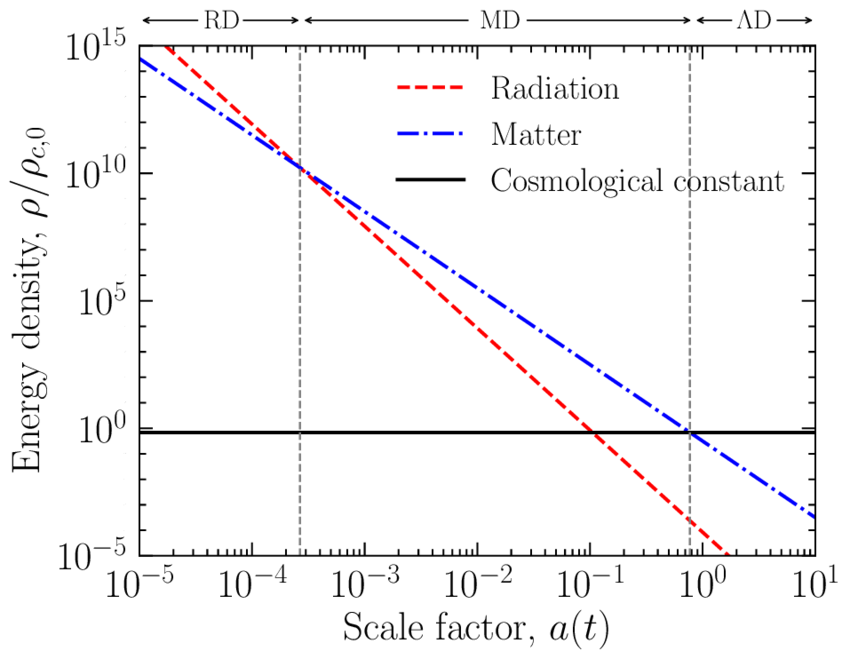
\includegraphics[width=\textwidth]{rho_vs_a}
\end{columns}
\end{frame}


% ============================================================
\section{The Cosmological Constant}
% ============================================================

% ---- Slide 32 ----------------------------------------------
\begin{frame}{Einstein's Static Universe}
\begin{itemize}
    \item In 1917, the prevailing view: the Universe is \emph{static}
    \item Problem: Friedmann equations do not admit a static solution for ordinary matter
    \item Setting $\dot{a}=0$ is possible, but then $\ddot{a}<0$ for $\rho+3p>0$ --- collapse is inevitable
    \item Einstein's fix: introduce a new constant $\Lambda$ that provides a repulsive term
\end{itemize}
\end{frame}

% ---- Slide 33 ----------------------------------------------
\begin{frame}{Modified Einstein Field Equations}
\begin{block}{Most general field equations}
\begin{equation*}
    G_{\mu\nu} + \Lambda\,g_{\mu\nu} = 8\pi G\,T_{\mu\nu}
\end{equation*}
\end{block}
\begin{itemize}
    \item $\Lambda g_{\mu\nu}$ is permitted because $\nabla_\alpha g_{\mu\nu}=0$
    \item Preserves Bianchi identity: $\nabla_\mu G^{\mu\nu}=0$
    \item Preserves energy--momentum conservation: $\nabla_\mu T^{\mu\nu}=0$
    \item $\Lambda$ is a \emph{geometrical constant of integration}
\end{itemize}
\end{frame}

% ---- Slide 34 ----------------------------------------------
\begin{frame}{Friedmann Equations with $\Lambda$}
\begin{alertblock}{First Friedmann Equation (with $\Lambda$)}
\begin{equation*}
    H^2 = \frac{8\pi G}{3}\,\rho - \frac{k}{a^2} + \frac{\Lambda}{3}
\end{equation*}
\end{alertblock}

\begin{alertblock}{Second Friedmann Equation (with $\Lambda$)}
\begin{equation*}
    \frac{\ddot{a}}{a} = -\frac{4\pi G}{3}(\rho+3p) + \frac{\Lambda}{3}
\end{equation*}
\end{alertblock}

$\Lambda>0$ contributes positively to $H^2$ and to $\ddot{a}/a$ --- it \textbf{accelerates} the expansion.
\end{frame}

% ---- Slide 35 ----------------------------------------------
\begin{frame}{Einstein's Static Universe: \alert{Unstable!}}
Set $\dot{a}=0$, $\ddot{a}=0$:
\begin{itemize}
    \item From 2nd Friedmann: $\Lambda=4\pi G(\rho+3p)$
    \item For dust ($p=0$): $\Lambda=4\pi G\rho$ and $k=4\pi G\rho\,a^2>0$ --- \textbf{closed} universe
\end{itemize}
\vspace{0.3cm}
\textbf{Instability:}
\begin{itemize}
    \item Perturb $a$ upward $\Rightarrow$ $\rho$ decreases ($\rho\propto a^{-3}$) but $\Lambda=\text{const}$
    \item Repulsion wins $\Rightarrow$ runaway expansion
    \item Small contraction $\Rightarrow$ gravity wins $\Rightarrow$ collapse
\end{itemize}
\vspace{0.2cm}
\begin{center}
\structure{Like a ball balanced on a hilltop}
\end{center}
\end{frame}

% ---- Slide 36 ----------------------------------------------
\begin{frame}{Vacuum Energy Interpretation}
Move $\Lambda$ to the right-hand side --- interpret as an effective fluid:
\begin{equation*}
    \rho_\Lambda = \frac{\Lambda}{8\pi G}\,,\qquad
    p_\Lambda = -\rho_\Lambda\,c^2
    \qquad\Longrightarrow\qquad w=-1
\end{equation*}
Density parameter:
\begin{equation*}
    \Omega_\Lambda = \frac{\rho_\Lambda}{\rho_{\rm crit}} = \frac{\Lambda}{3H^2}
\end{equation*}
\begin{itemize}
    \item QFT: vacuum zero-point fluctuations give a constant energy density
    \item But: QFT prediction overshoots by $\sim120$ orders of magnitude!
    \item One of the deepest unsolved problems in physics
\end{itemize}
\end{frame}

% ---- Slide 37 ----------------------------------------------
\begin{frame}{From ``Greatest Blunder'' to Dark Energy}
\begin{columns}[T]
\column{0.55\textwidth}
\begin{itemize}
    \item Hubble (1929): Universe is expanding --- motivation for $\Lambda$ evaporated
    \item Einstein called $\Lambda$ his ``greatest blunder''
    \item For most of 20th century: $\Lambda=0$
\end{itemize}
\vspace{0.2cm}
\pause
\alert{\textbf{1998:}} Riess et al.\ \& Perlmutter et al.\ --- Type Ia supernovae reveal \textbf{accelerating expansion}
\begin{itemize}
    \item Simplest explanation: $\Omega_{\Lambda,0}\approx 0.7$
    \item Foundation of the $\Lcdm$ model
\end{itemize}

\column{0.4\textwidth}
\vspace{0.3cm}
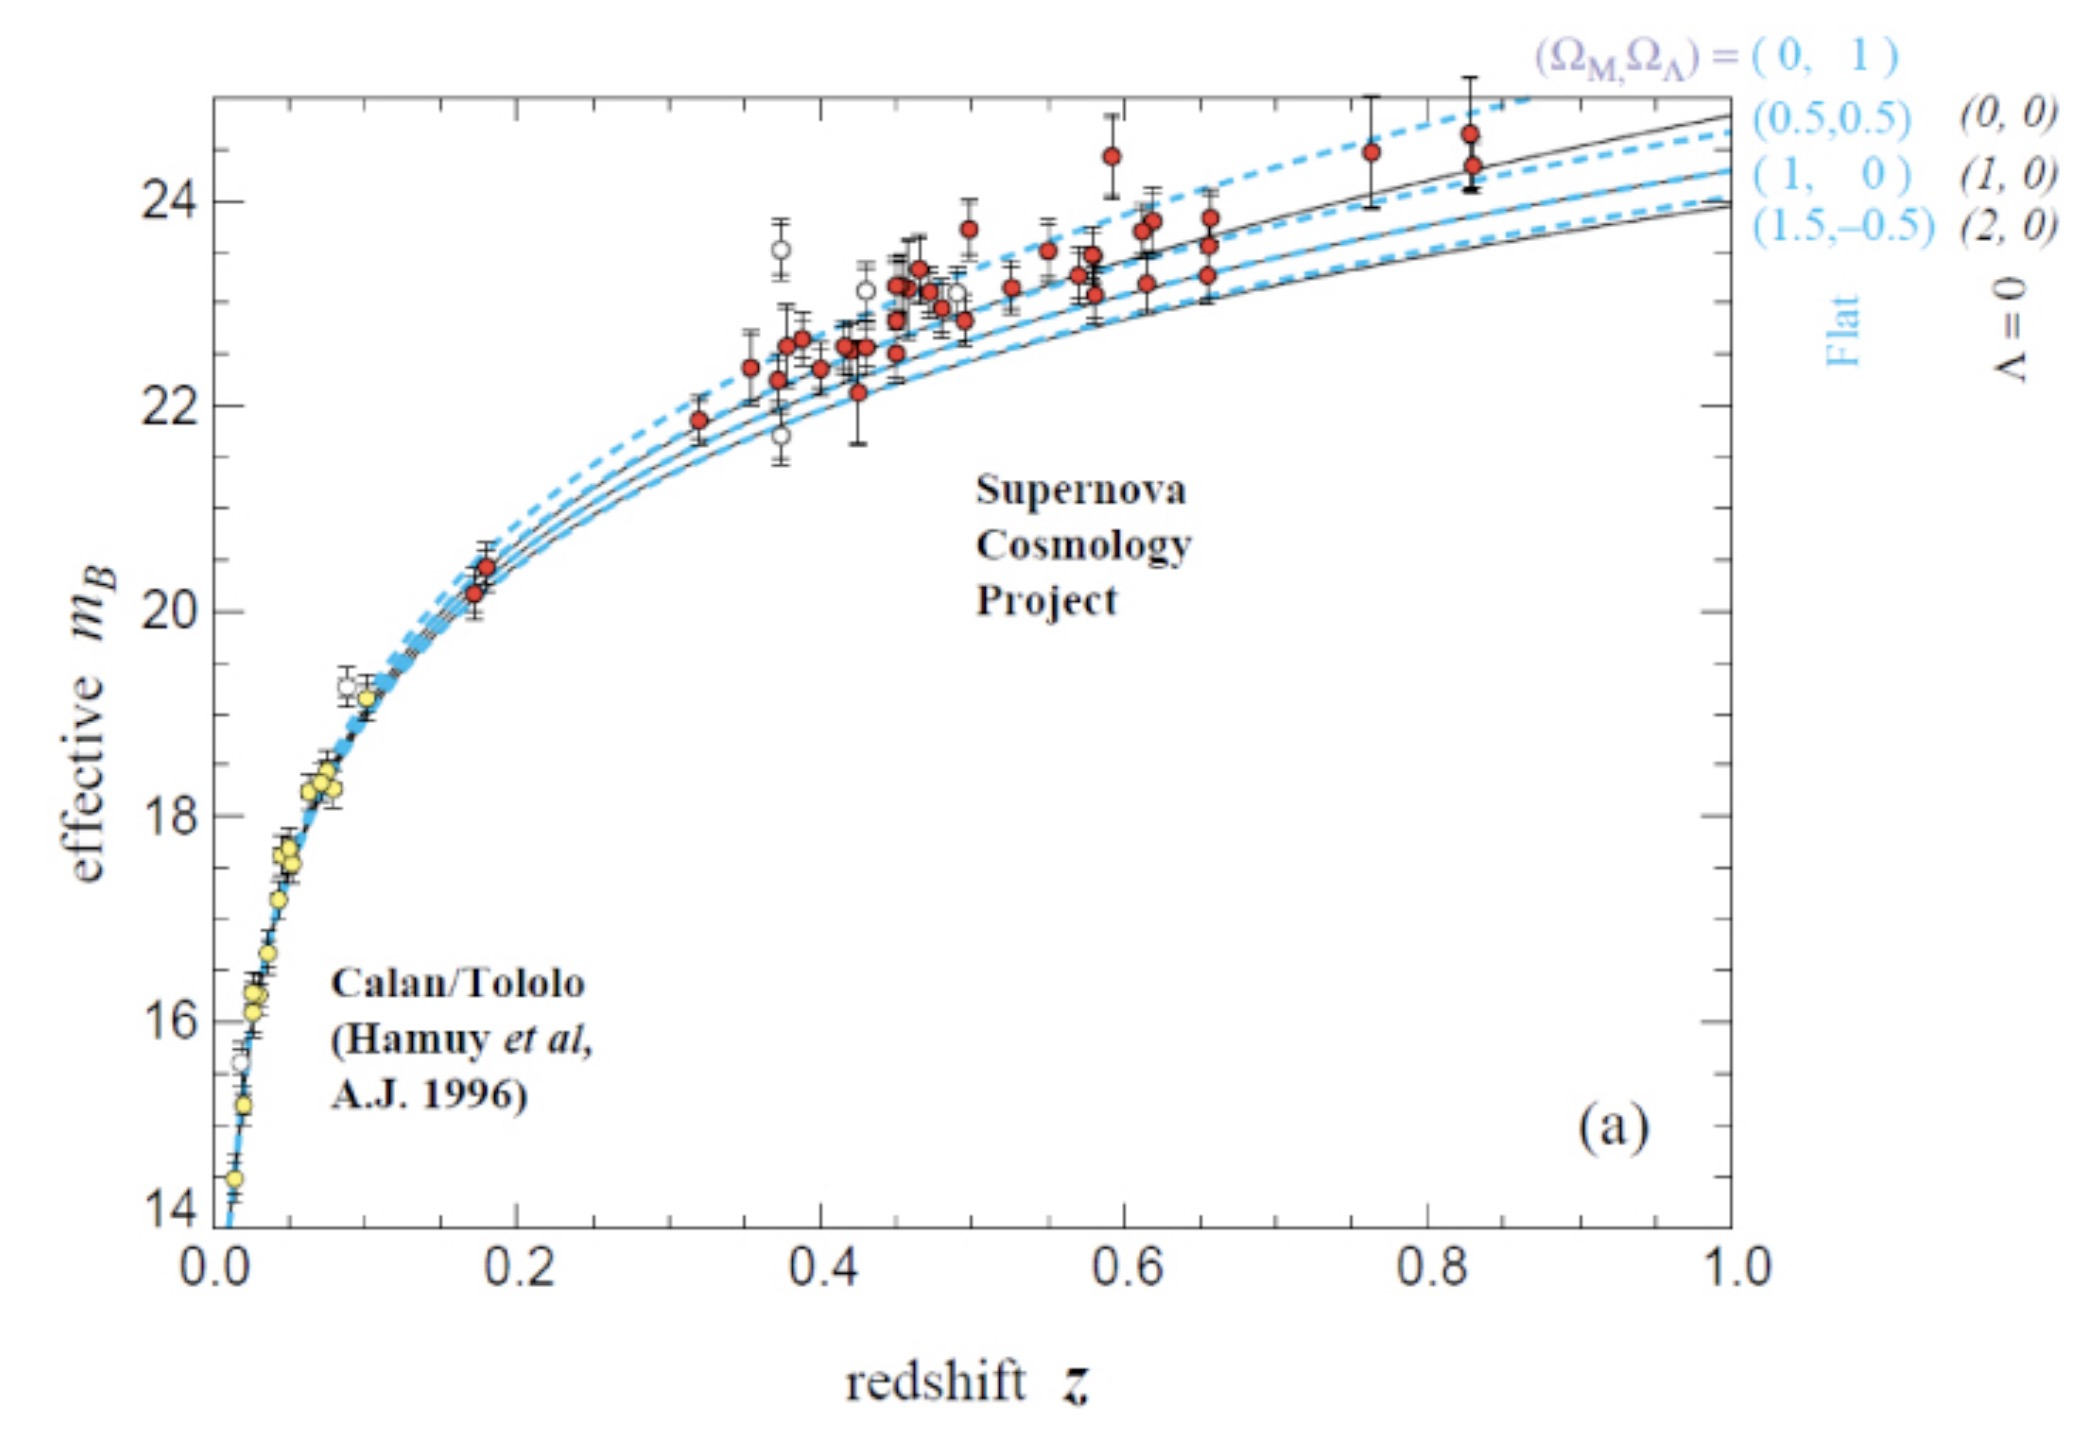
\includegraphics[width=\textwidth]{supernovae_evidence}
\end{columns}
\end{frame}


% ============================================================
\section{Solving the Friedmann Equations}
% ============================================================

% ---- Slide 38 ----------------------------------------------
\begin{frame}{Solving Friedmann: Roadmap}
We now solve the Friedmann equations for different contents and curvatures:
\begin{enumerate}
    \item Flat, matter-dominated (Einstein--de Sitter)
    \item Matter with curvature (open/closed)
    \item Flat, radiation-dominated
    \item Matter vs.\ radiation: which dominates when?
    \item Multiple components --- the general Friedmann integral
\end{enumerate}
\vspace{0.3cm}
Each case gives $a(t)$ --- the expansion history of the Universe.
\end{frame}

% ---- Slide 39 ----------------------------------------------
\begin{frame}{Flat Matter-Dominated Universe: Setup}
Matter density: $\rho_m = \rho_{m,0}/a^3$

\vspace{0.2cm}
Friedmann equation ($k=0$):
\begin{equation*}
    H^2 = \frac{8\pi G}{3}\,\frac{\rho_{m,0}}{a^3}
\end{equation*}
Take square root and define $A\equiv\sqrt{8\pi G\rho_{m,0}/3}$:
\begin{equation*}
    \dot{a} = A\,a^{-1/2}
\end{equation*}
Separable ODE:
\begin{equation*}
    a^{1/2}\,\dd a = A\,\dd t
\end{equation*}
\end{frame}

% ---- Slide 40 ----------------------------------------------
\begin{frame}{Einstein--de Sitter Solution}
Integrate with $a=0$ at $t=0$:
\begin{exampleblock}{Einstein--de Sitter ($k=0$, matter only)}
\begin{equation*}
    a(t) \propto t^{2/3}
\end{equation*}
\end{exampleblock}
\textbf{Properties:}
\begin{itemize}
    \item $H(t) = \dfrac{2}{3t}$
    \item Age: $t_0 = \dfrac{2}{3\Hnot}\approx 9.3$ Gyr \quad(\alert{too young!} Real age $\approx13.8$ Gyr)
    \item Deceleration parameter: $q\equiv -\dfrac{a\ddot{a}}{\dot{a}^2}=\frac{1}{2}$
    \item Expands forever but decelerates
\end{itemize}
\end{frame}

% ---- Slide 41 ----------------------------------------------
\begin{frame}{Matter + Curvature: Qualitative Behaviour}
\begin{columns}[T]
\column{0.55\textwidth}
Rewrite as an energy equation:
\begin{equation*}
    \dot{a}^2 = \frac{8\pi G\rho_{m,0}}{3}\,\frac{1}{a} - k
\end{equation*}
\begin{itemize}
    \item \textbf{Closed} ($k>0$): expansion halts at $a_{\rm max}$, then recollapses (``Big Crunch'')
    \item \textbf{Open} ($k<0$): expansion never halts; $a\propto t$ at late times
    \item \textbf{Flat} ($k=0$): borderline; $\dot{a}\to 0$ as $t\to\infty$
\end{itemize}

\column{0.4\textwidth}
\centering
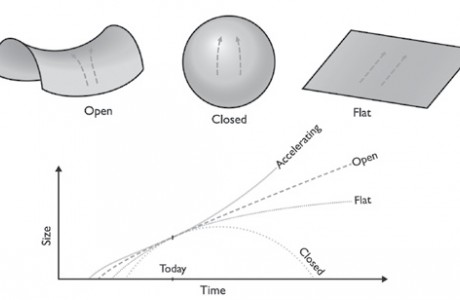
\includegraphics[width=\textwidth]{scale_factor_various_model}
\end{columns}
\end{frame}

% ---- Slide 42 ----------------------------------------------
\begin{frame}{Curvature and $\Omm$}
Evaluate Friedmann at $a=1$ today:
\begin{equation*}
    k = \Hnot^2\bigl(\Omega_{m,0}-1\bigr)
\end{equation*}
\begin{itemize}
    \item $\Omega_{m,0}=1\;\Rightarrow\;k=0$: flat (Einstein--de Sitter)
    \item $\Omega_{m,0}>1\;\Rightarrow\;k>0$: closed universe
    \item $\Omega_{m,0}<1\;\Rightarrow\;k<0$: open universe
\end{itemize}
\vspace{0.3cm}
The density parameter tells you the geometry!
\end{frame}

% ---- Slide 43 ----------------------------------------------
\begin{frame}{Parametric Solutions (Exact)}
\begin{columns}[T]
\column{0.46\textwidth}
\begin{block}{Closed ($k=+1$): cycloid}
\begin{align*}
    a &= \tfrac{a_{\rm max}}{2}(1-\cos\eta)\\[4pt]
    t &= \tfrac{a_{\rm max}}{2}(\eta-\sin\eta)
\end{align*}
$\eta: 0\to2\pi$ \newline
Big Bang $\to$ Big Crunch
\end{block}

\column{0.46\textwidth}
\begin{block}{Open ($k=-1$): hyperbolic}
\begin{align*}
    a &= \tfrac{a_0}{2}(\cosh\eta-1)\\[4pt]
    t &= \tfrac{a_0}{2}(\sinh\eta-\eta)
\end{align*}
Perpetual expansion
\end{block}
\end{columns}
\end{frame}

% ---- Slide 44 ----------------------------------------------
\begin{frame}{Radiation-Dominated Universe: Physics}
Consider a box of photons expanding with the Universe:

\vspace{0.3cm}
\textbf{Effect 1 --- Dilution:}
\begin{equation*}
    n \propto a^{-3} \qquad\text{(same as matter)}
\end{equation*}

\textbf{Effect 2 --- Redshift:}
\begin{equation*}
    \lambda\propto a \quad\Longrightarrow\quad
    E_\gamma = \frac{hc}{\lambda} \propto \frac{1}{a}
\end{equation*}

\textbf{Combined:}
\begin{equation*}
    \rho_r \propto n\cdot E_\gamma \propto a^{-3}\cdot a^{-1} = a^{-4}
\end{equation*}
\end{frame}

% ---- Slide 45 ----------------------------------------------
\begin{frame}{Radiation-Dominated Solution}
Friedmann ($k=0$): $H^2 = \frac{8\pi G}{3}\frac{\rho_{r,0}}{a^4}$

Separate and integrate:
\begin{exampleblock}{Radiation-dominated solution}
\begin{equation*}
    a(t) \propto t^{1/2}
\end{equation*}
\end{exampleblock}
\textbf{Properties:}
\begin{itemize}
    \item $H(t) = \dfrac{1}{2t}$
    \item Age: $t_0 = \dfrac{1}{2\Hnot}$ (even younger than EdS)
    \item $q=1$ (stronger deceleration than matter)
    \item Effective gravitational mass: $\rho+3p=2\rho$ for radiation
\end{itemize}
\end{frame}

% ---- Slide 46 ----------------------------------------------
\begin{frame}{Matter--Radiation Equality}
\begin{equation*}
    \frac{\rho_r}{\rho_m}
    = \frac{\rho_{r,0}}{\rho_{m,0}}\cdot\frac{1}{a}
\end{equation*}
\begin{itemize}
    \item Early times ($a\ll 1$): \textbf{radiation dominates}
    \item Late times ($a\gg a_{\rm eq}$): \textbf{matter dominates}
\end{itemize}
\vspace{0.3cm}
Crossover at matter--radiation equality:
\begin{equation*}
    a_{\rm eq} \approx \frac{1}{3400}\,,\qquad
    z_{\rm eq} \approx 3400\,,\qquad
    T_{\rm eq} \approx 9500\;\text{K}
\end{equation*}
Shortly before recombination ($z\approx 1100$).
\end{frame}

% ---- Slide 47 ----------------------------------------------
\begin{frame}{Thermal History in Brief}
\begin{columns}[T]
\column{0.45\textwidth}
Temperature scales as $T\propto 1/a$ (photon energy $\propto 1/a$).

\vspace{0.3cm}
\textbf{Two epochs:}
\begin{itemize}
    \item Early ($a\ll a_{\rm eq}$): radiation-dominated
    \begin{equation*}
        a\propto t^{1/2},\quad T\propto t^{-1/2}
    \end{equation*}
    \item After equality ($a\gg a_{\rm eq}$): matter-dominated
    \begin{equation*}
        a\propto t^{2/3},\quad T\propto t^{-2/3}
    \end{equation*}
\end{itemize}

\column{0.52\textwidth}
\centering
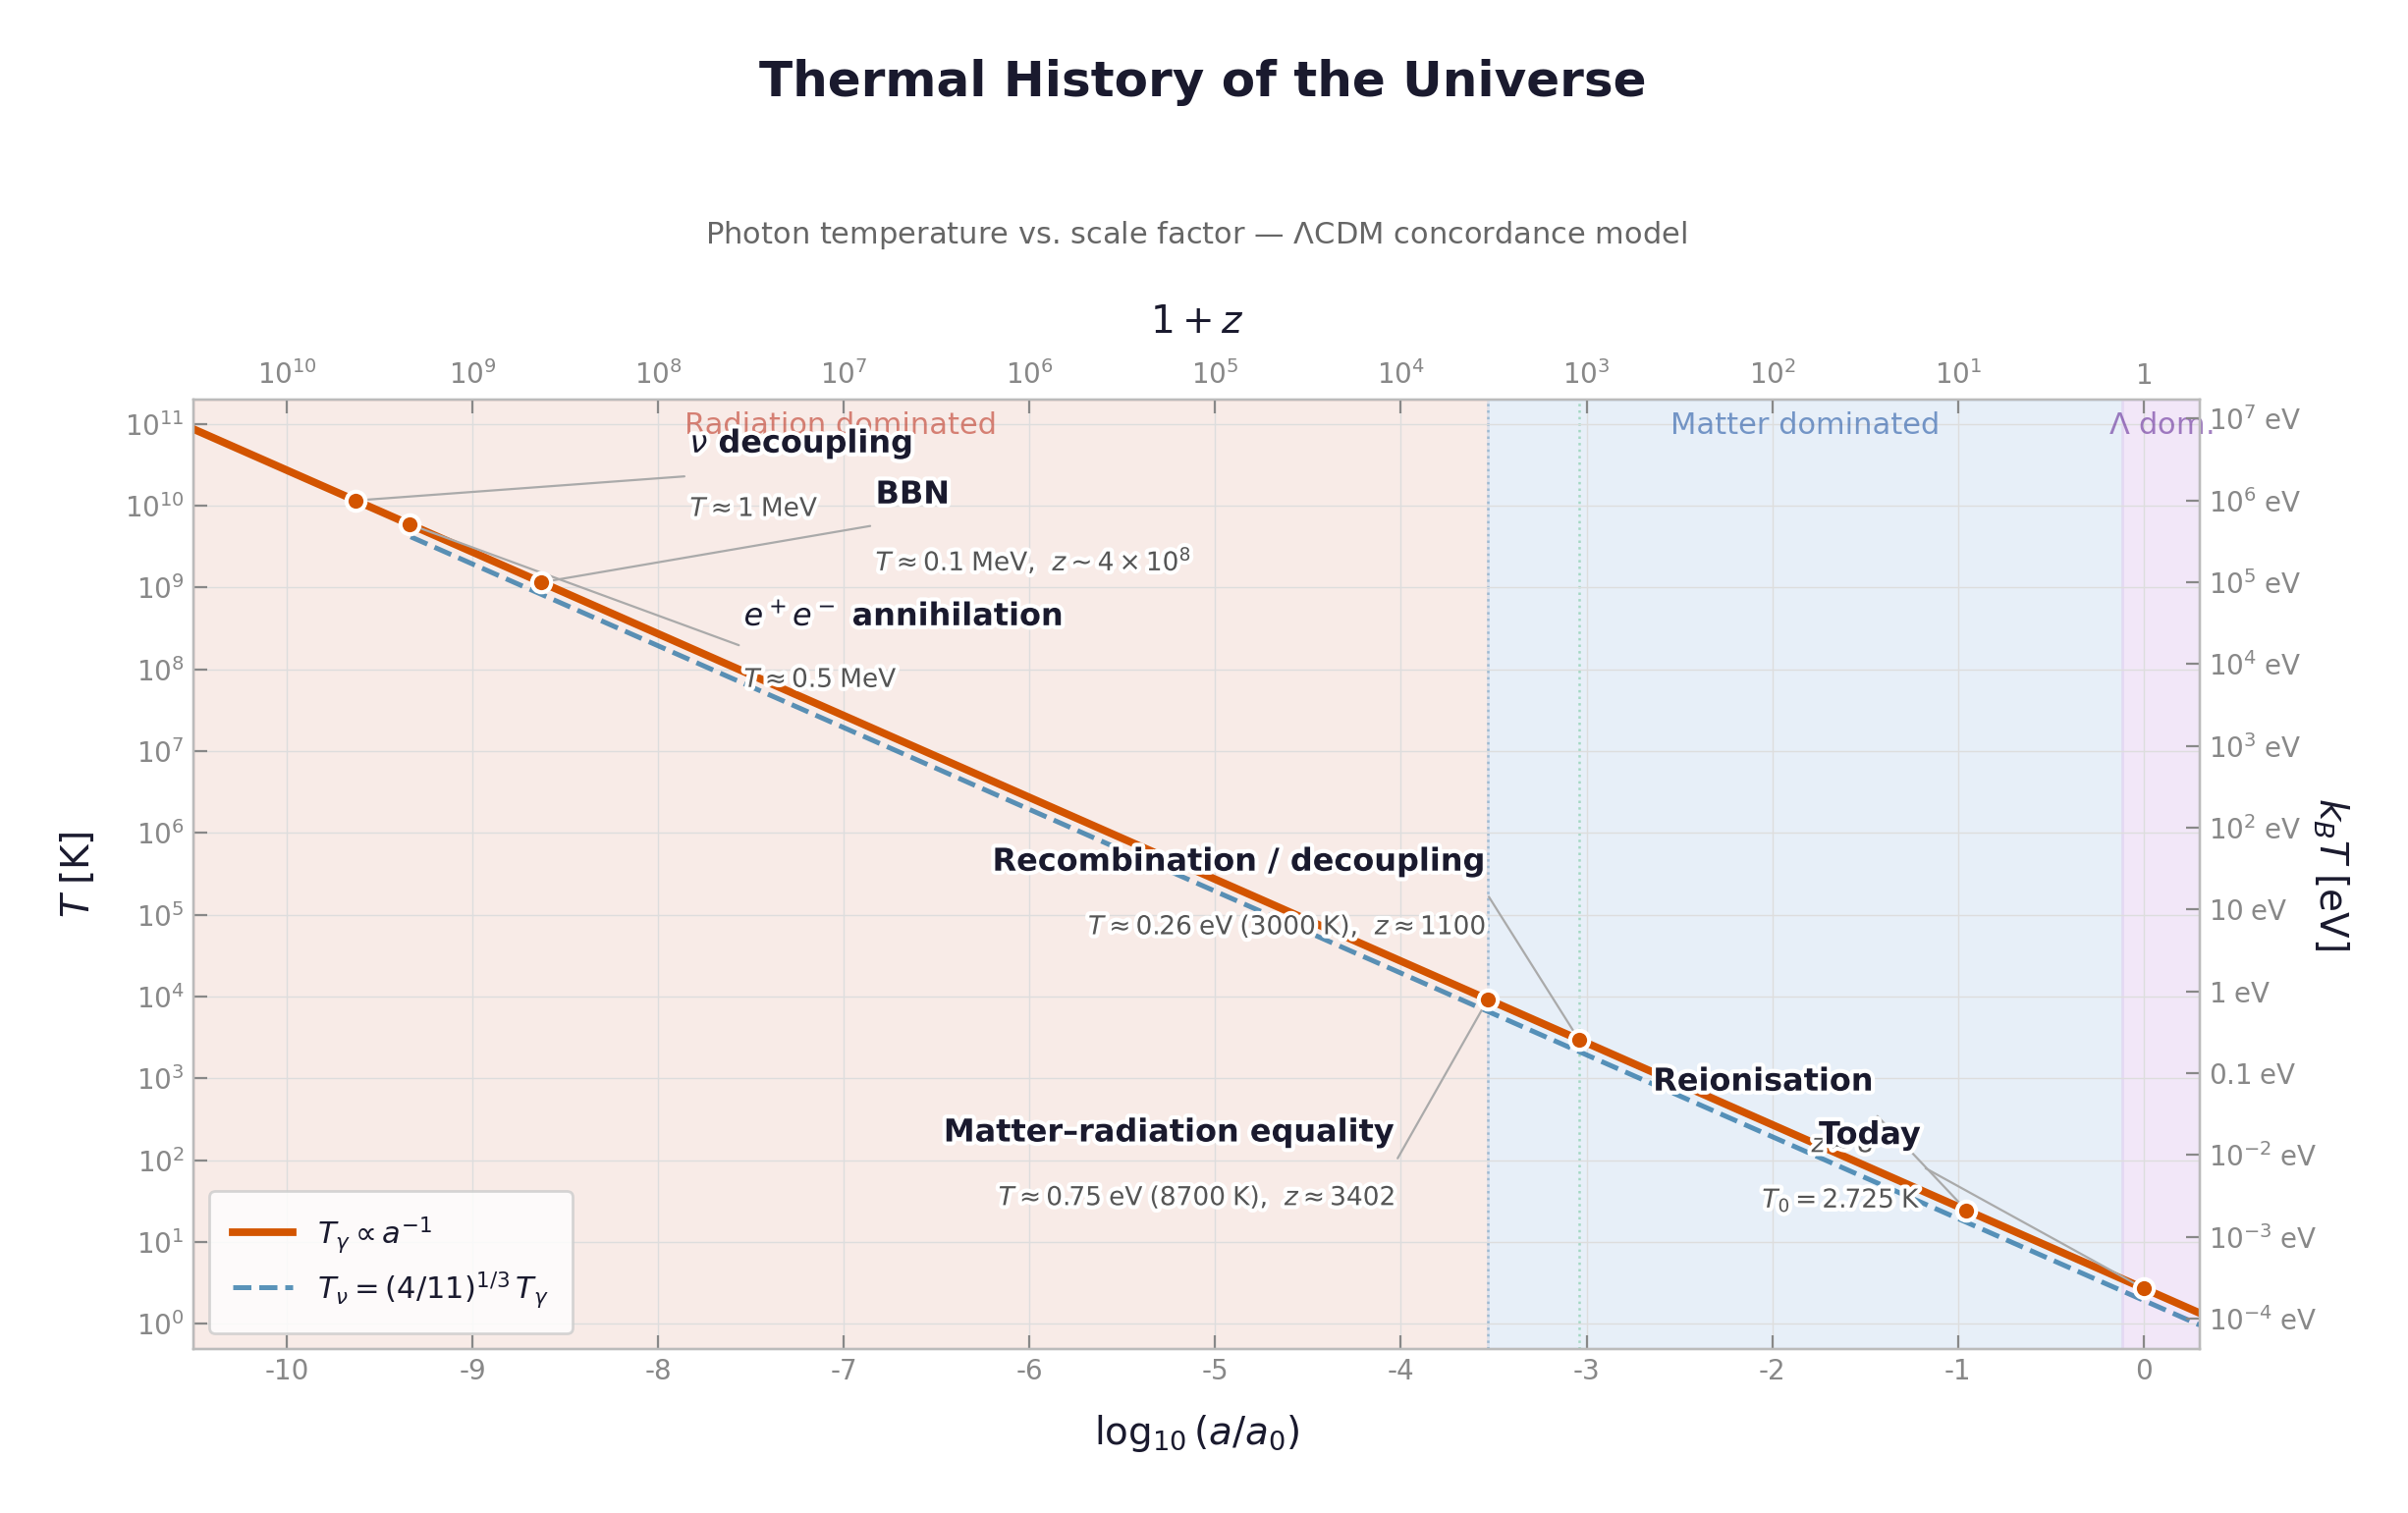
\includegraphics[width=\textwidth]{thermal_history_light}
\end{columns}
\end{frame}

% ---- Slide 48 ----------------------------------------------
\begin{frame}{Summary: Single-Component Flat Universes}
\small
General pattern: $\rho\propto a^{-3(1+w)}$, \;
$a(t)\propto t^{2/[3(1+w)]}$, \;
$H=\frac{2}{3(1+w)}\frac{1}{t}$, \;
$q=\frac{1+3w}{2}$

\vspace{0.3cm}
\begin{center}
\begin{tabular}{lcccccc}
\toprule
Component & $w$ & $\rho\propto$ & $a(t)\propto$ & $H(t)$ & $q$ & Age \\
\midrule
Matter    & $0$    & $a^{-3}$ & $t^{2/3}$ & $\frac{2}{3t}$ & $\frac{1}{2}$ & $\frac{2}{3\Hnot}$ \\[6pt]
Radiation & $\frac{1}{3}$  & $a^{-4}$ & $t^{1/2}$ & $\frac{1}{2t}$ & $1$ & $\frac{1}{2\Hnot}$ \\[6pt]
Curvature$^*$ & $-\frac{1}{3}$ & $a^{-2}$ & $t$ & $\frac{1}{t}$ & $0$ & $\frac{1}{\Hnot}$ \\[6pt]
$\Lambda$ & $-1$ & const & $\ee^{Ht}$ & const & $-1$ & $\infty$ \\
\bottomrule
\end{tabular}
\end{center}

\vspace{0.2cm}
\footnotesize $^*$``Curvature'' row: $k/a^2$ treated as effective fluid; empty coasting Milne universe.
\end{frame}

% ---- Slide 49 ----------------------------------------------
\begin{frame}{The Friedmann Integral}
For a flat universe with matter, radiation, and $\Lambda$:
\begin{equation*}
    H^2 = \Hnot^2\!\left[
    \frac{\Omega_{r,0}}{a^4}+\frac{\Omega_{m,0}}{a^3}+\Omega_{\Lambda,0}
    \right]
\end{equation*}
Age of the Universe:
\begin{alertblock}{}
\begin{equation*}
    t_0 = \frac{1}{\Hnot}\int_0^1
    \frac{\dd a}{\sqrt{\Omega_{r,0}\,a^{-2}+\Omega_{m,0}\,a^{-1}+\Omega_{\Lambda,0}\,a^2}}
\end{equation*}
\end{alertblock}
\begin{itemize}
    \item Generally requires numerical evaluation
    \item Reduces to analytic solutions in single-component limits
\end{itemize}
\end{frame}

% ---- Slide 50 ----------------------------------------------
\begin{frame}{The Age of the Universe}
\begin{columns}[T]
\column{0.55\textwidth}
Using observed values:\\
$\Omm\approx 0.3$, $\Omega_{\Lambda,0}\approx 0.7$, $\Omr\approx 10^{-4}$

\vspace{0.3cm}
\begin{exampleblock}{Result}
\begin{equation*}
    t_0 \approx 13.8\;\text{Gyr}
\end{equation*}
\end{exampleblock}

\vspace{0.2cm}
Compare:
\begin{itemize}
    \item Matter-only: $\sim9.3$ Gyr (too young)
    \item With $\Lambda$: $\sim13.8$ Gyr (\alert{correct!})
\end{itemize}

\column{0.4\textwidth}
\vspace{0.3cm}
\adjincludegraphics[width=\textwidth,trim={0 0 {.55\width} 0},clip]{cosmic_pie}
\end{columns}
\end{frame}


% ============================================================
\section{Summary}
% ============================================================

% ---- Slide 51 ----------------------------------------------
\begin{frame}{Summary: The Three Fundamental Equations}

\begin{alertblock}{First Friedmann Equation}
\vspace{-0.15cm}
\begin{equation*}
    H^2 = \frac{8\pi G}{3}\,\rho - \frac{k}{a^2} + \frac{\Lambda}{3}
\end{equation*}
\vspace{-0.3cm}
\end{alertblock}

\begin{alertblock}{Second Friedmann Equation}
\vspace{-0.15cm}
\begin{equation*}
    \frac{\ddot{a}}{a} = -\frac{4\pi G}{3}(\rho+3p) + \frac{\Lambda}{3}
\end{equation*}
\vspace{-0.3cm}
\end{alertblock}

\begin{alertblock}{Continuity Equation}
\vspace{-0.15cm}
\begin{equation*}
    \dot{\rho}+3H\!\left(\rho+\frac{p}{c^2}\right)=0
\end{equation*}
\vspace{-0.3cm}
\end{alertblock}

Only \textbf{two} of these three are independent. Together with $p=w\rho c^2$, they determine the full expansion history.
\end{frame}

% ---- Slide 52 ----------------------------------------------
\begin{frame}{Next Lecture: Dark Energy}
\begin{itemize}
    \item We derived the equations governing the expanding Universe
    \item Accelerating expansion requires $w<-1/3$
\end{itemize}
\vspace{0.3cm}
\textbf{Next time:}
\begin{itemize}
    \item Distances in an expanding Universe
    \item What is dark energy?
    \item Observational evidence beyond supernovae
    \item Is $w=-1$ exactly, or does it evolve?
    \item The $\Lcdm$ model in detail
\end{itemize}
\end{frame}

\end{document}
